%\title{Rapport_stage_M2}
%----------------------------------------------------------------------------------------
%	PACKAGES AND OTHER DOCUMENT CONFIGURATIONS
%----------------------------------------------------------------------------------------

\documentclass[12pt]{report}
\usepackage[english]{babel}
\usepackage[utf8x]{inputenc}
\usepackage[fleqn]{amsmath}
\usepackage{amssymb}
\usepackage{graphicx}
\usepackage[colorinlistoftodos]{todonotes}
\usepackage{geometry}
\geometry{hmargin=2.0cm,vmargin=1.5cm}
\usepackage{wrapfig}	% Figures avec du texte autour
\usepackage{lipsum}

\begin{document}

\begin{titlepage}

\newcommand{\HRule}{\rule{\linewidth}{0.5mm}} % Defines a new command for the horizontal lines, change thickness here

\center % Center everything on the page
 
%----------------------------------------------------------------------------------------
%	HEADING SECTIONS
%----------------------------------------------------------------------------------------
\textsc{\LARGE Le Mans Université}\\[1.5cm] % Name of your university/college
\textsc{\Large Rapport de Stage en Laboratoire}\\[0.5cm] % Major heading such as course name
\textsc{\large Master acoustique : Métiers de la recherche en acoustique}\\[0.5cm] % Minor heading such as course title

%----------------------------------------------------------------------------------------
%	TITLE SECTION
%----------------------------------------------------------------------------------------

\HRule \\[0.4cm]
{ \huge \bfseries Caractérisation et conception d'un milieu poreux anisotrope}\\[0.4cm] % Title of your document
\HRule \\[1cm]
 
%----------------------------------------------------------------------------------------
%	AUTHOR SECTION
%----------------------------------------------------------------------------------------

\begin{minipage}{0.4\textwidth}
\begin{flushleft} \Large
\emph{Author:}\\
Arthur \textsc{Terroir} % Your name
\end{flushleft}
\end{minipage}
~
\begin{minipage}{0.1\textwidth}
\end{minipage}
\begin{minipage}{0.5\textwidth}
\Large{\emph{Supervisor:} \\ Pr. Jean-Philippe \textsc{Groby}},\\
\large Chargé de Recherche CNRS.
\end{minipage}\\[1cm]

% If you don't want a supervisor, uncomment the two lines below and remove the section above
%\Large \emph{Author:}\\
%John \textsc{Smith}\\[3cm] % Your name

%----------------------------------------------------------------------------------------
%	DATE SECTION
%----------------------------------------------------------------------------------------

{\large \today}\\[1cm] % Date, change the \today to a set date if you want to be precise

%----------------------------------------------------------------------------------------
%	LOGO SECTION
%----------------------------------------------------------------------------------------
\hspace{2cm}
\begin{minipage}[c]{0.4\linewidth}
\centering
\hspace{-3cm}
\vspace{1.2cm}

\includegraphics[scale=0.9]{logo_LAUM.png}\\[1cm]  
\end{minipage}
\begin{minipage}[c]{0.4\linewidth}
\centering
\hspace{-1cm}
\vspace{1.2cm}

\includegraphics[scale=1.6]{logo_cnrs.jpg}\\[1cm]  
\end{minipage}
\begin{minipage}[l]{0.8\linewidth}
\centering
\hspace{1.3cm}
\vspace{0.5cm}

\includegraphics[scale=0.5]{Logo_LeMansUniv.png}\\[1cm]  
\end{minipage}
\end{titlepage}
%----------------------------------------------------------------------------------------
\begin{abstract}

\end{abstract}
\tableofcontents
\listoffigures

\newpage
\chapter*{Introduction}
\addcontentsline{toc}{chapter}{Introduction} 
\pagenumbering{arabic} \setcounter{page}{1}
   
%%%%%%%%%%%%%%%%%%%%%%%%%%%%%%%%%%%%%%%%%%%%%%%%%%%%%%%%%%%%%%%%%%%%%%%%%%%%%%%%%%%%%%%%%%%%%%%%%%%%%%%%%%%%% 
\chapter{Propagation dans une couche de fluide équivalent anisotrope}
\label{Ch_Prop}
\section{Problème de propagation dans le milieu fluide équivalent}
\label{Ch_Prop_S_Pb}
\subsection{Problème étudié}
\label{Ch_Prop_S_Pb_SS_Pb}
    Le problème étudié dans cette méthode est un problème de propagation dans un milieu fluide équivalent anisotrope, de dimension infinie dans le plan $x_1x_2$ et L selon $x_3$.  La situation est présentée sur la figure \ref{Schema}:
    \begin{figure}[ht!]
    \centering
    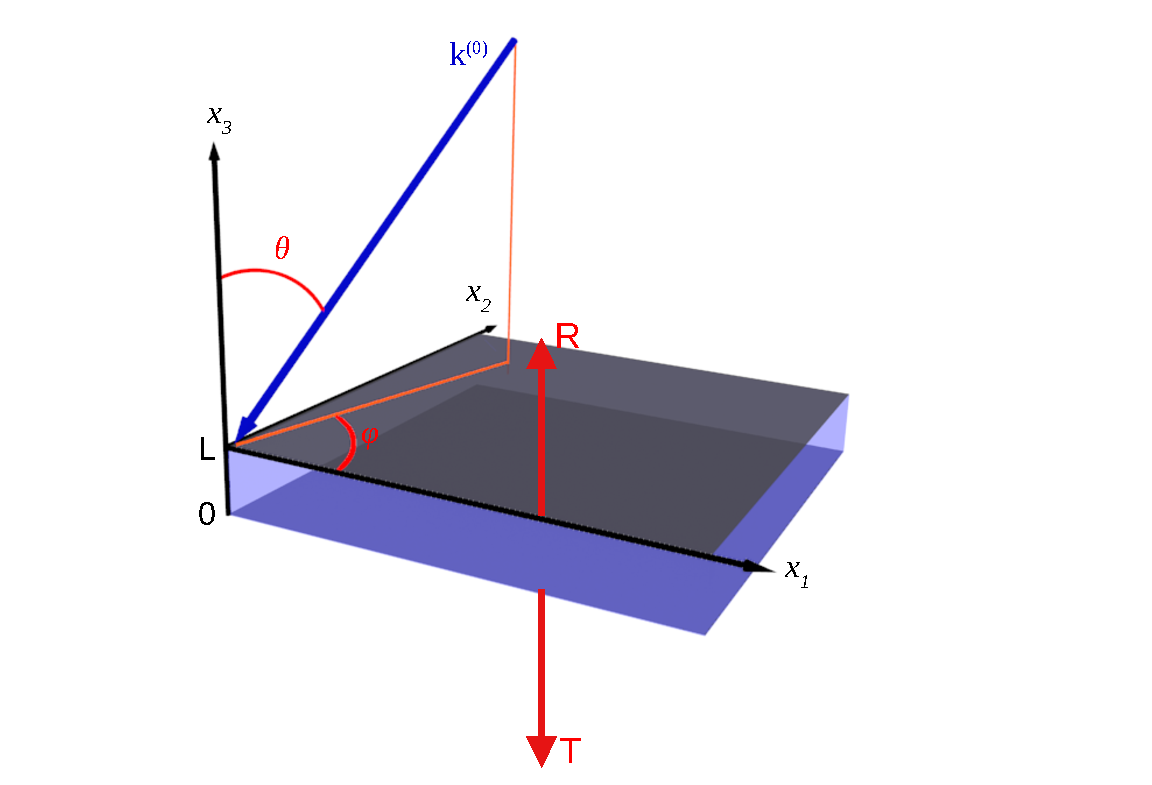
\includegraphics[scale=1]{Fig3D.eps}
    \caption{Réflexion et transmission dans un milieu fluide équivalent anisotrope. Le milieux est supposé infini dans le plan $x_1x_2$ et de dimension L selon $x_3$. Le fluide est excité avec une onde plane harmonique a l'interface $x_3=L$ et l'on observe une onde transmise en $x_3=0$. }
    \label{Schema}
    \end{figure}
    
    Dans ce problème on s'intéresse aux ondes réfléchies et transmises, soit au coefficients de réflexion et transmission R et T, pour une propagation le long de la direction $x_3$.
    Le fluide est considéré comme anisotrope et, dans le cas de notre étude, hors de ses directions principales. Le milieux étant un fluide équivalent, quelques observations sont a faire, dans un premier temps les grandeurs observées (bulk modulus, denisté) sont considérées comme complexe, due a la considération de perte. Dans un second temps, ces mêmes grandeurs sont dépendant de la fréquence.
    Il est donc possible de décrire la couche fluide avec une matrice de densité complexe telle que :
    \begin{align}
    \bar{\bar{\rho}}=\begin{pmatrix}
    					\rho_{11} & \rho_{12} & \rho_{13} \\
                        \rho_{12} & \rho_{22} & \rho_{23} \\
                        \rho_{13} & \rho_{23} & \rho_{33}                       
    				 \end{pmatrix}.
    \end{align},
    et d'un bulk modulus $K$.
    
    Le milieu est excité par une onde plane harmonique, d'amplitude 1, de pulsation $\omega$, d'angle d'incidence d'élévation $\theta$ et azimutal $\phi$. Les projections du nombre d'onde $k^{(0)}$ peuvent donc s'exprimer comme : 
        \begin{align}
        &k_1=-k_0 sin(\theta) cos(\phi), \\
        &k_2=-k_0 sin(\theta) sin(\phi), \\
        &k_3= -k_0 cos(\theta).
        \end{align}
        
        Le problème étant posé on s'intéresse maintenant au problème de propagation.
        
\subsection{Propagation dans le milieu fluide équivalent anisotrope}
\label{Ch_Prop_S_Pb_SS_Eul}
    Les équations constitutives suivantes sont considérées :
    \begin{align}
	&\rho \frac{\partial}{\partial t}v=-\nabla p,\label{Const1} \\
	&\frac{\partial}{\partial t}p=-K\nabla v.\label{Const2}
    \end{align}
    Les solutions a ces équations dans la couche fluide sont supposées être  des ondes plane harmonique telle que, en posant la convention temporelle $e^{i\omega t}$, l'on puisse écrire dans le domaine $0<x_3<L$ :
    \begin{align}
        \xi=\tilde{\xi}e^{i(k_1 x_1+k_2 x_2)}e^{-i\omega t}\label{Convention_k_t}
    \end{align}
    Le vecteur d'état $\bar{S}$ est ici introduit tel que $\bar{S}=\begin{pmatrix} p \\ v_3 \end{pmatrix}$, $\bar{S}$ permet de caractériser la propagation le long de la direction $x_3$, et ainsi d'obtenir la matrice de transfère $Tr$ du fluide entre les deux interfaces.
    
    En introduisant un champs de pression de la forme (\ref{Convention_k_t}) dans les équations (\ref{Const1}) et (\ref{Const2}), il vient :
    \begin{align}
	&ik_ip=\sum_{j=1}^{3} i \omega \rho_{ij} v_j,\ i=1,2\label{Euler1}\\
	&\frac{\partial}{\partial x_3}p=\sum_{j=1}^{3} i \omega \rho_{3j} v_j\label{Euler2}\\
    &i\omega p= iK(k_1v_1+k_2v_2+\frac{\partial}{\partial x_3}v_3).\label{Euler3}
    \end{align}
	En utilisant l'expression (\ref{Euler1}), il est possible d'écrire $v_1$ et $v_2$ en fonction de $p$ et $v_3$, comme :
    \begin{align}
	v_1=\frac{1}{\rho_{11}-\frac{\rho_{12}^2}{\rho_{22}}}([\frac{k_1}{\omega}-\frac{\rho_{12}}{\rho_{22}}\frac{k_2}{\omega}]p+[\frac{\rho_{12}}{\rho_{22}}\rho_{23}-\rho_{13}]v_3), \\
	v_2=\frac{1}{\rho_{22}-\frac{\rho_{12}^2}{\rho_{11}}}([\frac{k_2}{\omega}-\frac{\rho_{12}}{\rho_{11}}\frac{k_1}{\omega}]p+[\frac{\rho_{12}}{\rho_{11}}\rho_{13}-\rho_{23}]v_3).
    \end{align}
 	Ce qui permet d'exprimer $\frac{\partial}{\partial x_3}v_3$ et $\frac{\partial}{\partial x_3}p$ comme $\frac{\partial}{\partial x_3}v_3(p,v_3)$ et $\frac{\partial}{\partial x_3}p(p,v_3)$, en introduisant ces expressions dans les équations (\ref{Euler2}) et (\ref{Euler3}), il est donc possible d'écrire :
    \begin{align*}
    \frac{\partial}{\partial x_3}v_3=&[\frac{i\omega}{K}-\frac{ik_1}{\rho_{11}-\frac{\rho_{12}^2}{\rho_{22}}}(\frac{k_1}{\omega}-\frac{\rho_{12}}{\rho_{22}}\frac{k_2}{\omega})-\frac{ik_2}{\rho_{22}-\frac{\rho_{12}^2}{\rho_{11}}}(\frac{k_2}{\omega}-\frac{\rho_{12}}{\rho_{11}}\frac{k_1}{\omega})]p\\
    &-[\frac{ik_1}{\rho_{11}-\frac{\rho_{12}^2}{\rho_{22}}}(\frac{\rho_{12}}{\rho_{22}}\rho_{23}-\rho_{13})+\frac{ik_2}{\rho_{22}-\frac{\rho_{12}^2}{\rho_{11}}}(\frac{\rho_{12}}{\rho_{11}}\rho_{13}-\rho_{23})]v_3,
    \end{align*}
    et 
    \begin{align*}
    \frac{\partial}{\partial x_3}p=&[\frac{i\omega \rho_{13}}{\rho_{11}-\frac{\rho_{12}^2}{\rho_{22}}}(\frac{k_1}{\omega}-\frac{\rho_{12}}{\rho_{22}}\frac{k_2}{\omega})+\frac{i\omega \rho_{23}}{\rho_{22}-\frac{\rho_{12}^2}{\rho_{11}}}(\frac{k_2}{\omega}-\frac{\rho_{12}}{\rho_{11}}\frac{k_1}{\omega})]p\\
    &+[\frac{i\omega \rho_{13}}{\rho_{11}-\frac{\rho_{12}^2}{\rho_{22}}}(\frac{\rho_{12}}{\rho_{22}}\rho_{23}-\rho_{13})+\frac{i\omega \rho_{23}}{\rho_{22}-\frac{\rho_{12}^2}{\rho_{11}}}(\frac{\rho_{12}}{\rho_{11}}\rho_{13}-\rho_{23})]v_3.
    \end{align*}
    
    Sous forme matricielle, il est possible d'exprimer la matrice de propagation $\bar{\bar{A}}$ permettant de décrire l'évolution du vecteur d'état $\bar{S}$. Le problème de propagation prend donc la forme suivante :
    \begin{align}
    \frac{\partial}{\partial x_3}\bar{S} = \bar{\bar{A}} \bar{S},\label{Equa_diff}
    \end{align}
    avec $\bar{\bar{A}}$ la matrice de propagation telle que :
     \begin{align}
     &\bar{\bar{A}}=\begin{pmatrix}
    				A_{11} & A_{12} \\ A_{21} & A{22}
    			\end{pmatrix}\label{Matrice_complete},\\ 
     &A_{11}=A_{22}=i[\frac{\rho_2\rho_{13}-\rho_{12}\rho_{23}}{\rho_1\rho_2-\rho_{12}^2}k_1+\frac{\rho_1\rho_{23}-\rho_{12}\rho_{13}}{\rho_1\rho_2-\rho_{12}^2}k_2], \\
     &A_{12}=i\omega \rho_3[1-\frac{\rho_{13}}{\rho_1\rho_2-\rho_{12}^2}(\frac{k_1^{(i)}}{k_3^{(i)}})^2(\rho_2-\rho_{12}(\frac{k_2^{(i)}}{k_1^{(i)}})^2)-\frac{\rho_{23}}{\rho_1\rho_2-\rho_{12}^2}(\frac{k_2^{(i)}}{k_3^{(i)}})^2(\rho_1-\rho_{12}(\frac{k_1^{(i)}}{k_2^{(i)}})^2)], \\
     &A_{21}=\frac{i\omega}{K}[1-\frac{\rho_3}{\rho_1\rho_2-\rho_{12}^2}(\frac{k_1}{k_3^{(i)}})^2(\rho_2-\rho_{12}\frac{k_2}{k_1})-\frac{\rho_3}{\rho_1\rho_2-\rho_{12}^2}(\frac{k_2}{k_3^{(i)}})^2(\rho_1-\rho_{12}\frac{k_1}{k_2})],
    \end{align}
    ou $k_m^{(i)},\ i=1,2,3$ sont des nombre d'onde effectif selon la direction $x_i$, ne dépendant pas de la fréquence et de l'angle d'incidence.
    
	L'expression (\ref{Matrice_complete}) permet de décrire quatre paramètres liés à la propagation dans la couche fluide équivalente anisotrope, un Bulk modulus équivalent effectif $\tilde{K}$ liée a la direction de propagation et au Bulk modulus équivalent, une densité effective $\tilde{\rho_3}$ liée à la propagation des ondes selon $x_3$, et deux termes de phase $q_1$ et $q_2$, respectivement liés à $k_1$ et $k_2$, issus du couplage induit par les termes extra-diagonaux. Ces paramètres sont décrits ci-dessous :
    \begin{align}
     &\tilde{K}=\frac{K}{[1-\frac{\rho_{33}}{\rho_{11}\rho_{22}-\rho_{12}^2}(\frac{k_1}{k_3^{(i)}})^2(\rho_{22}-\rho_{12}\frac{k_2}{k_1})-\frac{\rho_{33}}{\rho_{11}\rho_{22}-\rho_{12}^2}(\frac{k_2}{k_3^{(i)}})^2(\rho_{11}-\rho_{12}\frac{k_1}{k_2})]}\label{Ktild},\\
     &\tilde{\rho_3}=\rho_{33}[1-\frac{\rho_{13}}{\rho_{11}\rho_{22}-\rho_{12}^2}(\frac{k_1^{(i)}}{k_3^{(i)}})^2(\rho_{22}-\rho_{12}(\frac{k_2^{(i)}}{k_1^{(i)}})^2)-\frac{\rho_{23}}{\rho_{11}\rho_{22}-\rho_{12}^2}(\frac{k_2^{(i)}}{k_3^{(i)}})^2(\rho_{11}-\rho_{12}(\frac{k_1^{(i)}}{k_2^{(i)}})^2)]\label{rho3tild}, \\
	&q_{1}=\frac{\rho_{22}\rho_{13}-\rho_{12}\rho_{23}}{\rho_{11}\rho_{22}-\rho_{12}^2}k_1\label{q1},\\
    &q_{2}= \frac{\rho_{11}\rho_{23}-\rho_{12}\rho_{13}}{\rho_{11}\rho_{22}-\rho_{12}^2}k_2\label{q2}.
          \end{align}
    Quelques commentaires peuvent être formulés a propos des ces paramètres, un premier point est que conformément a des paramètres effectif, dans un cas isotrope, l'on retrouve  $\tilde{K}=K$ et $\tilde{\rho_3}=\rho_3$. Il est possible de remarquer, que quelque soit l'anisotropie, en incidence normale, $\tilde{K}=K$. Une autre remarque importante est de voir que $\tilde{\rho_3}$ est indépendant de l'angle d'incidence de l'excitation, contrairement a $\tilde{K}$. Les termes de phase $q_1$ et $q_2$ semble traduire la variation de phase lors de la transmission de phase due au couplage induit par les densités extra-diagonales, et notamment $\rho_{13}$ et $\rho_{23}$  qu'on pourrai voir comme une rotation du plan principale $x_Ix_{II}$.
    
    Finalement, l'équation différentielle (\ref{Equa_diff}) amène à l'expression suivante : 
    \begin{align}
    \bar{S}_{(L)}=e^{\bar{\bar{A}}L}\bar{S}_{(0)}.\label{PB}
    \end{align}
    La matrice de transfère $Tr$ peut donc être déduite comme $Tr=e^{\bar{\bar{A}}L}$. Si l'expression analytique de la matrice de transfère est connue, c'est-a-dire que l'on puisse diagonaliser la matrice de propagation $\bar{\bar{A}}$, il est alors possible en posant des conditions au frontières de résoudre le problème réflexion/transmission dans le milieu fluide.
    
    Le calcul de la matrice de transfère du système passe donc par la diagonalisation de $\bar{\bar{A}}$, qui s'écrit :
    \begin{align}
    \bar{\bar{A}}=\bar{\bar{U}} \begin{pmatrix}
    								-ik_{33}+i\tilde{q} & 0 \\ 0 & ik_{33}+i\tilde{q} 
    							\end{pmatrix} \bar{\bar{U^{-1}}}.
    \end{align}
    avec $\tilde{q}=q_1+q_2$ le terme de phase global du système, $k_{33}=\frac{\omega}{c_{33}}$ le nombre d'onde effectif selon $x_3$, $c_{33}=\sqrt{\frac{\tilde{K}}{\tilde{\rho_3}}}$ la célérité dans la direction $x_3$.
    Les vecteurs propres s'écrivent :
    \begin{align}
    &\bar{\bar{U}}=\frac{1}{\sqrt{2}}\begin{pmatrix}
    					Z_3 & Z_3 \\ -1 & 1
    								\end{pmatrix},\\
    &\bar{\bar{U^{-1}}}=\frac{1}{Z_3 \sqrt{2}}\begin{pmatrix}
    					1 & -Z_3 \\ 1 & Z_3
    		   						\end{pmatrix},           
    \end{align}
    avec $Z_3=\tilde{\rho_3}c_{33}$ l'impédance effective du milieu fluide.
    La matrice de transfère $Tr$ peut donc s'écrire :
        \begin{align}
    Tr=\bar{\bar{U}}\begin{pmatrix}
    e^{-ik_{33}L} & 0 \\ 0 & e^{-ik_{33}L} 
    \end{pmatrix} e^{iq_1L}\bar{\bar{U^{-1}}}\label{Matrice_Transfere}
    \end{align}

\subsection{Conditions aux limites}
\label{Ch_Prop_S_Pb_SS_BC}
    La matrice de transfert du milieu étant connue, il faut donc maintenant poser des conditions frontière, dans notre problème on s'intéresse aux ondes réfléchies et transmises lors de la propagation d'une onde dans la couche fluide équivalentes anisotrope. Les conditions limites sont donc posées telles que :
    \begin{align}
    &\bar{S}_{x_3=L}=\bar{S}_{(L)}=\begin{pmatrix}
    						p_L \\ v_L
    					\end{pmatrix} = \begin{pmatrix}
    										1+R \\ -\frac{k_3}{\rho \omega}(1-R),
    									\end{pmatrix},\label{BC_L} \\
  	&\bar{S}_{x_3=0}=\bar{S}_{(0)}=\begin{pmatrix}
    						p_0 \\ v_0
    					\end{pmatrix} ==\begin{pmatrix}
    						T \\ -\frac{k_3}{\rho \omega}T,
    					\end{pmatrix}.\label{BC_0}
    \end{align}    
     Les conditions choisies aux interface $x_3=0$ et $x_3=L$, sont telle que les ondes réfléchies et transmises ai un phase nulle, autrement dit, il est considéré que les coefficients R et T contiennent une informations d'amplitude et de phase.    
        
\subsection{Problème à résoudre}    
    Si l'on introduit les expressions (\ref{Matrice_Transfere}), (\ref{BC_L}) et (\ref{BC_0}) dans l'équation (\ref{PB}), le problème de propagation peut donc s'écrire :
    \begin{align}
        \begin{pmatrix}
    	    1+R \\ -\frac{k_3}{\rho \omega}(1-R)
    	\end{pmatrix}=\bar{\bar{U}}\begin{pmatrix}
                        e^{-ik_{33}L} & 0 \\ 0 & e^{-ik_{33}L} 
                      \end{pmatrix} e^{i\tilde{q}L}\bar{\bar{U^{-1}}}\begin{pmatrix}
    					                            	T \\ -\frac{k_3}{\rho \omega}T
    				                                        	\end{pmatrix}.\label{Eq_Prop}
    \end{align}

    Le calcul de la fonction de transfert, et de R et T, peut être fait numériquement, en amont sans diagonaliser la matrice de propagation $\bar{\bar{A}}$, a partir de l'expression (\ref{Equa_diff}), mais cette méthode ne donne pas de forme analytique de ceci, ce qui ne permet pas d'établir une méthode inverse, et d'avoir des a priori sur R et T. C'est donc la dernière forme de l'équation de propagation (\ref{Eq_Prop}) qui est utilisé, pour dans un premier temps obtenir les coefficients de réflexion et transmissions pour une couche fluide anisotrope excité par une un onde plane harmonique, puis pour identifier les paramètres de la couche fluide par méthode inverse.
    
    On s'attachera dans les partie suivante à traiter le problème direct, la détermination de R et T connaissant le fluide. Puis l'identification des paramètres du fluide équivalent (densité et bulk modulus) connaissant R et T pour différents angles d'incidence. Finalement un validation numérique de la méthode est faite dans le cas d'une couche de matériau poreux, homogénéisé en fluide équivalent par le modèle Jhonson-Champoux-Allard-Lafarge (citation). 
    
   %%%%%%%%%%%%%%%%%%%%%%%%%%%%%%%%%%%%%%%%%%%%%%%%%%%%%%%%%%%%%%%%%%%%%%%%%%%%%%%%%%%%%%%%%%%%%%%%%%%%%%%%%%%%%%%%%%%%%%%%%%%%%%%%%%%%%%%%%%%%%%%%%%%%%%%%%%%%%%%%%%%%%%%%%%%%%%%%%%%%%%%%%%%%%%%%%%%%%%%%%%%%%%%%%%%%%%%%%%%%%%%%%%%%%%%%%%%%%%%%%%%%%%%%%%%%%%%%%%%%
\chapter{Problème direct : coefficient de réflexion et transmission R et T}
\label{Ch_Dir}
    Les  coefficients R et T peuvent être récupérer de deux manières différentes, numériquement, avec le calcul de l'exponentiel $e^{\bar{\bar{A}}L}$ de matrice connaissant la matrice de propagation $\bar{\bar{A}}$, et analytiquement en résolvant l'équation (\ref{Eq_Prop}).
    
    Il est proposé ici de déterminer l'expression analytique de R et T, qui dans la suite  pourra donner des a priori sur les signaux étudiés lors de la méthode de propagation inverse. 

\section{Coefficients de Réflexion/transmission R et T}
\label{Ch_Dir_S_R/T}
    Les paramètres du fluides équivalent (\ref{Ktild}), (\ref{rho3tild}), (\ref{q1}) et (\ref{q2}) sont ici rappelés :
    \begin{align*}
    &\tilde{K}=\frac{K}{[1-\frac{\rho_3}{\rho_1\rho_2-\rho_{12}^2}(\frac{k_1}{k_3^{(i)}})^2(\rho_2-\rho_{12}\frac{k_2}{k_1})-\frac{\rho_3}{\rho_1\rho_2-\rho_{12}^2}(\frac{k_2}{k_3^{(i)}})^2(\rho_1-\rho_{12}\frac{k_1}{k_2})]},\\
    &\tilde{\rho_3}=\rho_3[1-\frac{\rho_{13}}{\rho_1\rho_2-\rho_{12}^2}(\frac{k_1^{(i)}}{k_3^{(i)}})^2(\rho_2-\rho_{12}(\frac{k_2^{(i)}}{k_1^{(i)}})^2)-\frac{\rho_{23}}{\rho_{1}\rho_2-\rho_{12}^2}(\frac{k_2^{(i)}}{k_3^{(i)}})^2(\rho_1-\rho_{12}(\frac{k_1^{(i)}}{k_2^{(i)}})^2)], \\
    &\tilde{q}=q_1+q_2,\\
    &q_{1}=\frac{\rho_2\rho_{13}-\rho_{12}\rho_{23}}{\rho_1\rho_2-\rho_{12}^2}k_1,\\
    &q_{2}= \frac{\rho_1\rho_{23}-\rho_{12}\rho_{13}}{\rho_1\rho_2-\rho_{12}^2}k_2.
    \end{align*}
    
    L'équation de propagation (\ref{Eq_Prop}) peut être réécrite comme :
    \begin{align}
         \bar{\bar{U^{-1}}}\bar{S}_{(L)}=\begin{pmatrix}
                        e^{-ik_{33}L} & 0 \\ 0 & e^{-ik_{33}L} 
                      \end{pmatrix} e^{i\tilde{q}L}\bar{\bar{U^{-1}}}\bar{S}_{(0)},
    \end{align}
    ce qui devient en développant :
    \begin{align}
    \begin{pmatrix}
		p_L-Z_3v_L \\ p_L+Z_3v_L
    \end{pmatrix}=\begin{pmatrix}
              		(p_0-Z_3v_0)e^{-i k_{33} L} \\ (p_0+Z_3v_0)e^{i k_{33} L}
            \end{pmatrix} e^{i \tilde{q} L}\label{eqDif_tmp}
    \end{align}  
    
    R et T peuvent être obtenus avec la résolution du système de 2 équations a 2 inconnues, en rappelant les conditions aux limites (\ref{BC_L}) et (\ref{BC_0}), tels que :
    \begin{align}
    &T=\frac{e^{-i\tilde{q}L}}{cos(k_{33}L)-\frac{i}{2}(\frac{Z}{Z_3}+\frac{Z_3}{Z})sin(k_{33}L)}\label{Transmission},\\ 
    &R=\frac{i}{2} \frac{(\frac{Z}{Z_3}-\frac{Z_3}{Z})sin(k_{33}L)}{cos(k_{33}L)-\frac{i}{2}(\frac{Z_3}{Z}+\frac{Z}{Z_3})sin(k_{33}L)}\label{Reflexion}.
    \end{align}
    
    Il est possible de voir dans l'expression (\ref{Transmission}) que $\tilde{q}$ induit une variation de phase dans le coefficient de réflexion, variation qui dépend des densités complexes du milieu fluide, et donc de l'anisotropie du milieu. Dans le cas particulier où les densités $\rho_{13}$ et $\rho_{23}$ soit nulles, $\tilde{q}$ est nul, et donc il n'y aura aucun changement de la phase de T. Autrement dit, si l'on assimile les deux densités précédentes a des rotations du plan principale $\rho_I\rho_{II}$, $\tilde{q}$ traduit le déphasage induit par l'anisotropie du nouveau plan du matériau $x_1x_2$. De plus, comme attendu, $k_{33}$ joue bien le rôle d'un nombre d'onde effectif.
    
\section{Comparaison analytique et numérique}
\label{Ch_Dir_S_Comp}
    Afin de valider les expressions (\ref{Reflexion}) et (\ref{Transmission}) de R et T, il est ici proposé de comparer les R et T obtenus analytiquement et numériquement, pour des densités et un bulk modulus dépendant de la fréquence. Les densités complexes, le bulk modulus ainsi que les coefficients R et T obtenus en incidence normale sont représentés sur la figure (\ref{RT_comp}) :
\begin{figure}[ht!]
    \centering
    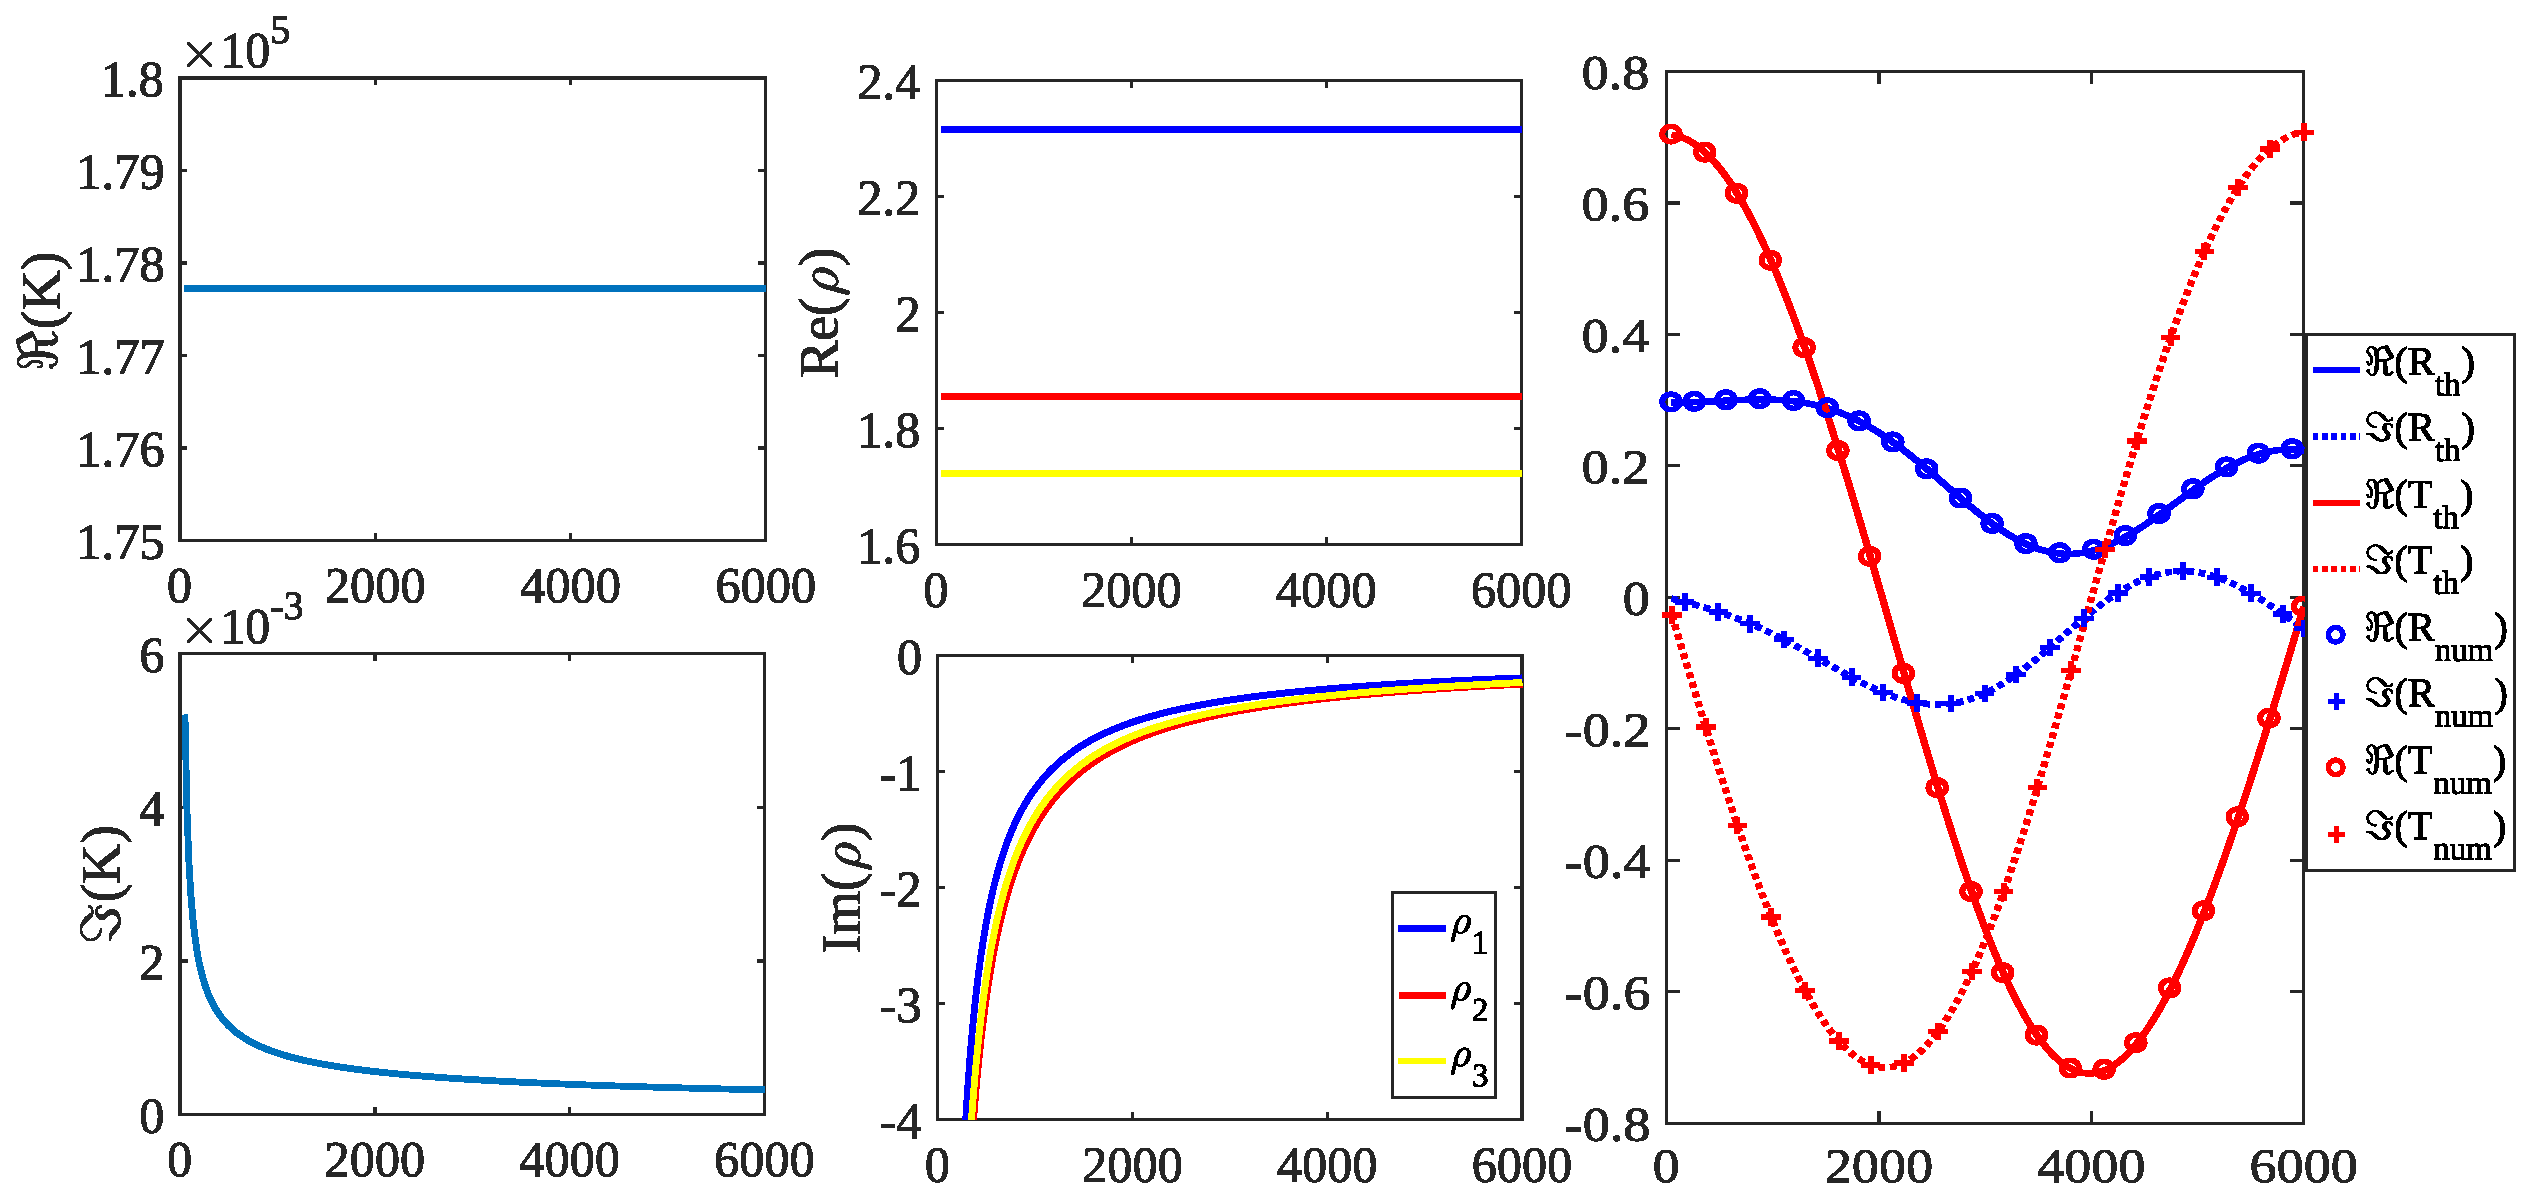
\includegraphics[scale=0.4]{RT_num_th.eps}
    \caption{ Coefficients de transmission et réflexion (colonne 3) obtenus par un calcul numérique et analytique de la matrice de transfère $Tr$ du milieu fluide équivalent. Les paramètres du fluides équivalent sont le bulk modulus complexe (colonne 1) et les 3 densités principales complexes (colonne 2). Une concordance parfaite est observé pour les R et T calculés numériquement et analytiquement.}
    \label{RT_comp}
\end{figure}
    
    Un concordance parfaite est obtenue pour les coefficients R et T en incidence normale, pour toutes les fréquences du domaine étudié. La validation des expressions (\ref{Transmission}) et (\ref{Reflexion}) est donc concluante. 

%%%%%%%%%%%%%%%%%%%%%%%%%%%%%%%%%%%%%%%%%%%%%%%%%%%%%%%%%%%%%%%%%%%%%%%%%%%%%%%%%%%%%%%%%%%%%%%%%%%%%%%%%%%%%%%%%%%%%%%%%%%%%%%%%%%%%%%%%%%%%%%%%%%%%%%%%%%%%%%%%%%%%%%%%%%%%%%%%%%%%%%%%%%%%%%%%%%%%%%%%%%%%%%%%%%%%%%%%%%%%%%%%%%%%%%%%%%%%%%%%%%%%%%%%%%%%%%%%%%%
\chapter{Problème inverse : Détermination de la matrice de densité $\bar{\bar{\rho}}$ et du Bulk modulus équivalent $\tilde{K}$}
\label{Ch_Inv}
	L'étude du problème direct étant maintenant faites, il est proposé de reprendre la relation (\ref{PB}) de propagation a travers la couche fluide, connaissant l'expression de la matrice de transfère $e^{\bar{\bar{A}}L}$, et de mettre en place une méthode inverse permettant de retrouver les densités complexes et le Bulk modulus effectif a partir des coefficients R et T.
    
    Cette méthode est développée, comme pour le calcul direct, avec des cas de complexité croissante. Cette approche nous offre une compréhension plus aisée des mécanisme mis en jeu lors de la résolution inverse et nous permet au final de voir une résolution simplifiée dans le cas général. 
    Afin de reconstruire les différentes densités à partir des coefficients R et T, il est nécessaire d'avoir autant d'information que de densités a déterminer. Pour avoir différentes informations en utilisant les coefficients de réflexion et de transmission, il existe plusieurs solution, ici il est proposé de faire varier l'angle d'incidence de l'onde se propageant dans le milieu poreux. Ainsi pour chaque incidence, on observe deux coefficients R et T, il est donc possible théoriquement de résoudre le problème inverse si l'on mesure R et T à autant d'angle d'incidence que de densités a déterminer. 
    
    La première étude de la propagation d'une onde harmonique a travers la couche de fluide équivalent nous a permis d'obtenir la matrice de transfert correspondante a la propagation dans le milieu dans les différents cas que l'on va voir. De plus il est maintenant possible de poser des hypothèses sur R et T, connaissant leur forme analytiques, ce qui est utilisé dans la résolution du problème inverse.
    
    la méthode inverse est appliquée au cas de la propagation dans la couche fluide équivalente anisotrope selon le même plan que pour l'étude direct, partant d'un milieu disposé selon ses directions principales jusqu'à voir le cas où il est disposé de manière totalement arbitraire. Dans les différents cas où l'on ne considère pas une anisotropie complète, on supposera le bulk modulus comme connu, et son obtention ne sera présenté que pour le cas le plus général, quand le matériau est complètement anisotrope.
    
    La résolution se basant sur l'angle d'incidence  de l'onde harmonique se propageant dans le milieu, il est rappeler ici que le problème étudié est représenté sur le schéma (\ref{Schema}), où l'on considère les nombre d'onde suivant :
    \begin{align*}
    &k_1=-k_0 sin(\theta) cos(\phi), \\
    &k_2=-k_0 sin(\theta) sin(\phi), \\
    &k_3= -k_0 cos(\theta).
    \end{align*} 
    



%%%%%%%%%%%%%%%%%%%%%%%%%%%%%%%%%%%%%%%%%%%%%%%%%%%%%%%%%%%%%%%%%%%%%%%%%%%%%%%%%%%%%%%%%%%%%%%%%%%%%%%%%%%%%%%%%%%%
Le dernier cas traité est le cas où l'on considère une rotation des 3 directions principales selon les directions $x_1$, $x_2$ et $x_3$. Le problème est donc un couplage des différents cas de rotations indépendantes vus précédemment, il est donc logique que l'on retrouve les deux méthodes de résolution du problème de propagation inverse afin de récupérer la matrice densité a partir des coefficients R et T. Un nouveau paramètre a déterminer est introduit dans cette section, a savoir que dans les sections précédentes le Bulk modulus effectif été supposé connu, or si l'on ne connaît pas le matériaux poreux, il est aussi a déterminer. La méthode inverse devra donc maintenant déterminer les densités complexes ainsi que le Bulk modulus effectif du milieu.    
    
    Il est proposé de présenter la méthode dans le cas général, où le matériau modélisé en fluide équivalent anisotrope est totalement inconnu, par sa symétrie et son Bulk modulus effectif. Cette méthode reprend les mêmes principes que les méthodes développée précédemment avec dans un premier temps l'obtention des termes de phase $q_1$ et $q_2$, définissant ainsi F(R,T), puis résolvant un système de 3 équations a inconnues. Une étape supplémentaire est la détermination du Bulk modulus effectif, possible connaissant $Z_3$ et $\tilde{\rho_3}$.
    
    La matrice de densité complexe est complète dans le cas où la symétrie de la couche fluide anisotrope n'est pas connu, les paramètres de la matrice de propagation  sont rappelés par les expressions (\ref{Ktild}), (\ref{rho3tild}), (\ref{q1}) et \ref{q2}) :
     \begin{align*}
	 &\bar{\bar{\rho}}=\begin{pmatrix} \rho_1 & \rho_{12} & \rho_{13} \\ \rho_{12} & \rho_2 & \rho_{23} \\ \rho_{13} & \rho_{23} & \rho_3 \end{pmatrix},\\
     &\bar{\bar{A}}=\begin{pmatrix} i \tilde{q} & i \omega \tilde{\rho_3} \\ \frac{i \omega}{\tilde{K}} & i \tilde{q} \end{pmatrix},\\
	 &\tilde{K}=\frac{K}{[1-\frac{\rho_{33}}{\rho_{11}\rho_{22}-\rho_{12}^2}(\frac{k_1}{k_3^{(i)}})^2(\rho_{22}-\rho_{12}\frac{k_2}{k_1})-\frac{\rho_{33}}{\rho_{11}\rho_{22}-\rho_{12}^2}(\frac{k_2}{k_3^{(i)}})^2(\rho_{11}-\rho_{12}\frac{k_1}{k_2})]},\\
     &\tilde{\rho_3}=\rho_{33}[1-\frac{\rho_{13}}{\rho_{11}\rho_{22}-\rho_{12}^2}(\frac{k_1^{(i)}}{k_3^{(i)}})^2(\rho_{22}-\rho_{12}(\frac{k_2^{(i)}}{k_1^{(i)}})^2)-\frac{\rho_{23}}{\rho_{11}\rho_{22}-\rho_{12}^2}(\frac{k_2^{(i)}}{k_3^{(i)}})^2(\rho_{11}-\rho_{12}(\frac{k_1^{(i)}}{k_2^{(i)}})^2)], \\
     &\tilde{q}=q_1+q_2,\\
	 &q_{1}=\frac{\rho_{22}\rho_{13}-\rho_{12}\rho_{23}}{\rho_{11}\rho_{22}-\rho_{12}^2}k_1,\\
     &q_{2}= \frac{\rho_{11}\rho_{23}-\rho_{12}\rho_{13}}{\rho_{11}\rho_{22}-\rho_{12}^2}k_2.
          \end{align*}
          
\subsection{Impédance effective $Z_3$ et fonction F(R,T)}
	Conformément à la section (\ref{Ch_Inv_S_rho13/23_SS_F(R,T)}), il est possible d'écrire l'impédance effective $Z_3$ a partir du problème de propagation entre les deux interfaces (\ref{PB}) telle que :
    \begin{align*}
    &Z_3=F(R,T,\tilde{q})Z,\nonumber\\
    &F(R,T,\tilde{q})=\sqrt{\frac{T^2e^{2i\tilde{q}l}-(1+R)^2}{T^2e^{2i\tilde{q}L}-(1-R)^2}}.
    \end{align*}
    Cette fonction est connu et défini en incidence normale, la où l'on sait que le terme de phase $\tilde{q}$ s'annule. Pour la connaître en tout point, et donc pouvoir définir l'impédance $Z_3$, $\tilde{q}$ doit être identifié. 
    
\subsection{Bulk modulus équivalent $\tilde{K}$}
   	L'identification du Bulk modulus équivalent $\tilde{K}$ se a partir de la définition de l'impédance effective $z_3$, elle peut être définit comme $Z_3=\tilde{\rho_3}c_{33}$. La célérité effective des ondes dans le milieu fluide peut se définir de deux façons différentes, en fonction des propriété effective du milieu, $c_{33}=\sqrt{\frac{\tilde{K}}{\tilde{\rho_3}}}$, ou en fonction du nombre d'onde effectif dans le milieu, $c_{33}=\frac{\omega}{k_{33}}$. Connaissant $Z_3$ en incidence normale, il suffit d'obtenir le nombre d'onde effectif $k_{33}$, afin de connaître $\tilde{K}$ et $\tilde{\rho_3}$.
    
    $k_{33}$ peut être déduit du problème de propagation (\ref{PB}), dans ce cas $Z_3$ est supposée connue et l'on cherche a identifier le nombre d'onde effectif en incidence normale. En repartant de l'expression matricielle de l'équation de propagation entre les deux interfaces, il est possible d'écrire la relation (\ref{Eq_diff_matr2}), avec les conditions aux limites (\ref{BC_0}) et (\ref{BC_L}), comme :
    \begin{align*}
    e^{i k_{33}L}=\frac{(1+R)-\frac{Z_3}{Z}(1-R)}{T-\frac{Z_3}{Z}T},
    \intertext{En incidence normale, le terme de phase $\tilde{q}$ est nulle et l'impédance $Z_3$ est connue soit :}
    e^{i k_{33}L}=\frac{Z(1+R)-Z_3(1-R)}{(Z-Z_3)T}.
    \end{align*}
    
    Maintenant que $k_{33}$ est déterminer, la célérité effective des ondes $c_{33}$ est connue, l'on peut simplement obtenir $K$ et $\tilde{\rho_3}$, en considérant $\tilde{K}=K$ en incidence normale, par :
    \begin{align*}
    &K=\frac{Z_3}{k_{33}}^{\theta=0}_{\phi=0},\\
    &\tilde{\rho_3}=\frac{Z_3 k_{33}}{\omega}^{\theta=0}_{\phi=0}.
    \end{align*}
    
\subsection{Système d'équation}
	Le calcul de $\tilde{K}$ dans la section précédente permet de poser l'impédance effective $Z_3$ comme un système d'équation dépendant des deux angles d'incidences en reprenant la méthode utilisée dans la partie (\ref{Ch_Inv_S_rho13_SS_rho2}). En posant $\tilde{K}=\frac{K}{\alpha}$ et $\tilde{\rho_3}=\rho_3 \beta$, il est possible d'écrire :
    \begin{align}
    &\alpha=1-\frac{K}{\omega^2}\frac{\rho_2 k_1^2+\rho_1 k_2^2-2\rho_{12}k_1k_2}{\rho_1\rho_2-\rho_{12}^2},\nonumber \\
    &\beta=1-\frac{\rho_{13}(\rho_2\rho_{13}-\rho_{12}\rho_{23})+\rho_{23}(\rho_1\rho_{23}-\rho_{12}\rho_{13})}{\rho_3(\rho_1\rho_2-\rho_{12}^2)},\nonumber \\
    &\gamma=\frac{K}{Z_3^2},\nonumber \\
    &\frac{1}{\rho_3}\frac{\alpha}{\beta}=\frac{1-\frac{K}{\omega^2}\frac{\rho_2 k_1^2+\rho_1 k_2^2-2\rho_{12}k_1k_2}{\rho_1\rho_2-\rho_{12}^2}}{\rho_3-\frac{\rho_{13}(\rho_2\rho_{13}-\rho_{12}\rho_{23})+\rho_{23}(\rho_1\rho_{23}-\rho_{12}\rho_{13})}{\rho_1\rho_2-\rho_{12}^2}}=\gamma.\label{alpha_beta_complet}
    \end{align}
    
    Six densités sont a déterminer par la méthode inverse, il faut donc logiquement les coefficient R et T pour 6 incidences différentes, les informations de R et T étant contenues dans l'impédance $Z_3$ et donc $\gamma$. 
	Les informations nécessaires peuvent se décomposer selon quatre catégories :
    \begin{itemize}
    \item Une information en incidence normale afin de déterminer $\tilde{K}$ et $\tilde{\rho_3}$, et ainsi de connaître la densité $\rho_3$. 
    \item Deux informations selon l'axe $x_1$ afin de pouvoir déterminer le terme de phase $q_1$ par une variation de phase des coefficient de transmission
    \item Deux informations selon $x_2$ pour déterminer le terme de phase $q_2$
    \item Une information en incidence oblique afin de pouvoir résoudre le système de 3 équations a 3 inconnues conformément a la section (\ref{Ch_Inv_S_rho12_SS_rho1/2/12}) et de pouvoir déterminer $\rho_1$, $\rho_2$ et $\rho_{12}$ 
    \end{itemize}
    
    Les six équations issue de la relation (\ref{alpha_beta_complet}) qui nous intéresse sont, en reprenant la notation indicielle des angles :
    \begin{align}
    \intertext{En incidence normale : $\theta=0$, $\phi=0$}
    &\frac{1}{\tilde{\rho_3}}=\frac{1}{\rho_3-\frac{\rho_{13}(\rho_2\rho_{13}-\rho_{12}\rho_{23})+\rho_{23}(\rho_1\rho_{23}-\rho_{12}\rho_{13})}{\rho_1\rho_2-\rho_{12}^2}}=\Large{\gamma|}^{(0)}_{(0)},\ \tilde{q}=0,\label{Eq_complet_0_0}
    \intertext{En incidence orienté selon l'axe $x_1$ : $\theta=\frac{\pi}{6}$, $\phi=0$ et $\theta=\frac{-\pi}{6}$, $\phi=0$}
    &\frac{1}{\tilde{\rho_3}}[1-\frac{K}{\omega^2}\frac{\rho_2}{\rho_1\rho_2-\rho_{12}^2}k_1^2]=\Large{\gamma|}^{(\frac{\pi}{6})}_{(0)},\ \tilde{q}=\frac{-1}{2}q_1^{(0)},\ q_1^{(0)}=\frac{\rho_2\rho_{13}-\rho_{12}\rho_{23}}{\rho_1\rho_2-\rho_{12}^2}k^{(0)}\label{Eq_complet_pi6_0}\\
    &\frac{1}{\tilde{\rho_3}}[1-\frac{K}{\omega^2}\frac{\rho_2}{\rho_1\rho_2-\rho_{12}^2}k_1^2]=\Large{\gamma|}^{(\frac{-\pi}{6})}_{(0)},\ \tilde{q}=-\frac{1}{2}q_1^{(0)}\label{Eq_complet_-pi6_0}\\
    \intertext{En incidence orienté selon l'axe $x_2$ : $\theta=\frac{\pi}{6}$, $\phi=\frac{\pi}{2}$ et $\theta=\frac{-\pi}{6}$, $\phi=\frac{\pi}{2}$}
    &\frac{1}{\tilde{\rho_3}}[1-\frac{K}{\omega^2}\frac{\rho_1}{\rho_1\rho_2-\rho_{12}^2}k_2^2]=\Large{\gamma|}^{(\frac{\pi}{6})}_{(\frac{\pi}{2})},\ \tilde{q}=\frac{-1}{2}q_2^{(0)},\ q_2^{(0)}=\frac{\rho_1\rho_{23}-\rho_{12}\rho_{13}}{\rho_1\rho_2-\rho_{12}^2}k^{(0)}\label{Eq_complet_pi6_pi2}\\
    &\frac{1}{\tilde{\rho_3}}[1-\frac{K}{\omega^2}\frac{\rho_1}{\rho_1\rho_2-\rho_{12}^2}k_2^2]=\Large{\gamma|}^{(\frac{-\pi}{6})}_{(\frac{\pi}{2})},\ \tilde{q}=\frac{1}{2}q_2^{(0)},\label{Eq_complet_-pi6_pi2}\\
    \intertext{En incidence oblique : $\theta=\frac{\pi}{4}$, $\phi=\frac{\pi}{4}$ }
    &\frac{1}{\tilde{\rho_3}}[1-\frac{K}{\omega^2}\frac{\rho_1+\rho_2-2\rho_{12}}{\rho_1\rho_2-\rho_{12}^2}k^2]=\Large{\gamma|}^{(\frac{\pi}{4})}_{(\frac{\pi}{4})},\ \tilde{q}=\frac{-1}{2}q_1^{(0)}+\frac{-1}{2}q_2^{(0)},\ k=k_1=k_2\label{Eq_complet_pi4_pi4}\\
    \end{align}
    
\subsection{Terme de phase $\tilde{q}=q_1+q_2$}
	La première étape dans l'identification des densités complexes, connaissant le bulk modulus équivalent, est l'obtention des termes de phase $q_1$ et $q_2$ comme fait dans la section (\ref{Ch_Inv_S_rho13/23}) traitant de deux rotation azimutales des directions principales. Ces termes connus, il est possible d'avoir l'impédance $Z_3$ en tout points. 
    
    Contrairement a la section (\ref{Ch_Inv_S_rho13/23}), il n'est plus possible de déterminer $q_1$ et $q_2$ grâce a une information en incidence oblique de part le couplage induit par la densité $\rho_{12}$. Il est donc proposé une nouvelle méthode, utilisant la variation de phase des coefficients de transmission et de réflexion  pour deux ondes ayant une incidence différente le long de l'axe $x_1$ ou $x_2$. Il est possible de cette façon de mettre en évidence les terme de phase correspondant $q_1$ et $q_2$.
    
\subsubsection*{Terme de phase $q_1$}
	La différence d'impédance $\Gamma$ pour deux d'incidence le long de $x_1$ peut s'écrire $\Gamma=\gamma|^{(\frac{\pi}{6})}_{(0)}-\gamma|^{(\frac{-\pi}{6})}_{(0)}$.
	En remplaçant par les expressions (\ref{Eq_complet_pi6_0}) et (\ref{Eq_complet_-pi6_0}), il vient $\Gamma=0$, et l'on peut développer en rappelant que $\gamma=\frac{K}{Z_3^2}=\frac{K}{(F(R,T,\tilde{q})Z)^2}$ :
    \begin{align*}
    \frac{K}{F^2(R,T,\tilde{q})Z^2}|^{(\frac{\pi}{6})}_{(0)}-\frac{K}{F^2(R,T,\tilde{q})Z^2}|^{(\frac{-\pi}{6})}_{(0)}=0
    \end{align*}
    
    Cette expression peut être simplifier, dans un premier temps il est facile de remarquer que l'impédance Z est la même pour les deux angles, $k_3$ étant le même dans les deux cas. La seconde simplification possible vient du fait que la différence d'angle de propagation n'induit qu'un changement sur le terme de phase $q_1$ et donc sur T, on a donc $R=R|^{(\frac{\pi}{6})}_{(0)}=R|^{(\frac{-\pi}{6})}_{(0)}$. 
	
    L'expression peut se réécrire, avec les notations $X=X|^{(\frac{\pi}{6})}_{(0)}$ et $X'=X|^{(\frac{-\pi}{6})}_{(0)}$ :
    \begin{align*}
    \frac{T^2e^{-iq_1^{(0)}L}-(1-R)^2}{T^2e^{-iq_1^{(0)}L}-(1+R)^2}-\frac{T'^2e^{iq_1^{(0)}L}-(1-R)^2}{T'^2e^{iq_1^{(0)}L}-(1+R)^2}=0,
    \end{align*}
    d'où en mettant au dénominateur commun :
    \begin{align*}
    &[T^2e^{-iq_1^{(0)}L}-(1-R)^2][T'^2e^{iq_1^{(0)}L}-(1+R)^2]-[T^2e^{-iq_1^{(0)}L}-(1+R)^2][T'^2e^{iq_1^{(0)}L}-(1-R)^2]=0,\\
    \leftrightarrow & [(1+R)^2+(1-R)^2]T^2e^{-iq_1^{(0)}L}+[(1+R)^2-(1-R)^2]T'^2e^{iq_1^{(0)}L}=0,\\
    \leftrightarrow & -4RT^2e^{-iq_1^{(0)}L}+4RT'^2e^{iq_1^{(0)}L}=0. 
    \end{align*}
    
    Il est donc finalement possible d'écrire le terme de phase $q_1$ a partir de l'expression (\ref{q10L_complet}) que l'on sait déterminer :
    \begin{align}
    e^{iq_1^{(0)}L}=\frac{T}{T'}=\frac{T|^{(\frac{\pi}{6})}_{(0)}}{T|^{(\frac{-\pi}{6})}_{(0)}} \label{q10L_complet}
    \end{align}

\subsubsection*{Terme de phase $q_2$}
	De façon analogue il est possible de montrer qu'en prenant une différence d'impédance $Z_3$ pour des angles d'incidence le long $x_2$ telle que $\Gamma'=\gamma|^{(\frac{\pi}{6})}_{(\frac{\pi}{2})}-\gamma|^{(\frac{-\pi}{6})}_{(\frac{\pi}{2})}$, l'on peut retrouver $q_2$ par le même calcul :
    \begin{align}
    e^{iq_2^{(0)}L}=\frac{T|^{(\frac{\pi}{6})}_{(\frac{\pi}{2})}}{T|^{(\frac{-\pi}{6})}_{(\frac{\pi}{2})}} \label{q20L_complet}
    \end{align}
        

\subsection{Densités $\rho_1$, $\rho_2$ et $\rho_{12}$}
	Les deux termes de phase étant identifier, il est possible de connaître l'impédance $Z_3$ pour tout les angles d'incidence, et la résolution se ramène aux problème du cas orthotrope faites dans la partie (\ref{Ch_Inv_S_rho12}).
    L'identification des densités $\rho_1$, $rho_2$ et $rho_{12}$ passe donc la résolution d'un système de 3 équation a 3 inconnues conformément a la section (\ref{Ch_Inv_S_rho12_SS_rho1/2/12}.
    
    Il est proposé de réécrire le système d'équation pour faire isoler les différentes densités a déterminer, les trois nouvelles équations provenant des expressions (\ref{Eq_complet_pi6_0}), (\ref{Eq_complet_pi6_pi2}) et (\ref{Eq_complet_pi4_pi4}) sont :
    \begin{align}
    (\ref{Eq_complet_pi6_0}) \leftrightarrow\ &\frac{K}{\omega^2}\frac{\rho_2}{\rho_1\rho_2-\rho_{12}^2}k_1^2=[1-\tilde{\rho_3}\gamma|^{(\frac{\pi}{6})}_{(0)}]=\gamma'|^{(\frac{\pi}{6})}_{(0)}\label{Comp_1},\\
    (\ref{Eq_complet_pi6_pi2}) \leftrightarrow\ &\frac{K}{\omega^2}\frac{\rho_1}{\rho_1\rho_2-\rho_{12}^2}k_2^2=[1-\tilde{\rho_3}\gamma|^{(\frac{\pi}{6})}_{(\frac{\pi}{2})}]=\gamma'|^{(\frac{\pi}{6})}_{(\frac{\pi}{2})}\label{Comp_2},\\
    (\ref{Eq_complet_pi4_pi4}) \leftrightarrow\ &\frac{K}{\omega^2}\frac{\rho_1+\rho_2-2\rho_{12}}{\rho_1\rho_2-\rho_{12}^2}k^2=[1-\tilde{\rho_3}\gamma|^{(\frac{\pi}{4})}_{(\frac{\pi}{4})}]=\gamma'|^{(\frac{\pi}{4})}_{(\frac{\pi}{4})}\label{Comp_3}.
    \end{align}
    
    Pour les 3 expressions (\ref{Comp_1}), (\ref{Comp_2}) et (\ref{Comp_3}), les projection des nombres d'ondes sont les même, autrement dit, $k=k_1=k_2$ pour tout les angles d'incidence choisis.
    En utilisant ces relations, trois rapports de densité peuvent être écrit , tels que :
    \begin{align}
    &\frac{(\ref{Comp_2})}{(\ref{Comp_1})} :\ \frac{\rho_1}{\rho_2}=\frac{\gamma'|^{(\frac{\pi}{6})}_{(0)}}{\gamma'|^{(\frac{\pi}{6})}_{(\frac{\pi}{2})}}=X_1,\label{Comp_rho2_rho1} \\
    &\frac{(\ref{Comp_1})+(\ref{Comp_2})-(\ref{Comp_3})}{(\ref{Comp_2})} :\ \frac{\rho_{12}}{\rho_1}=\frac{1}{2}\frac{\gamma'|^{(\frac{\pi}{6})}_{(0)}+\gamma'|^{(\frac{\pi}{6})}_{(\frac{\pi}{2})}-\gamma'|^{(\frac{\pi}{4})}_{(\frac{\pi}{4})}}{\gamma'|^{(\frac{\pi}{6})}_{(\frac{\pi}{2})}}=X_2,\label{Comp_rho12_rho1} \\
    &\frac{(\ref{Comp_1})+(\ref{Comp_2})-(\ref{Comp_3})}{(\ref{Comp_1})} :\ \frac{\rho_{12}}{\rho_2}=\frac{1}{2}\frac{\gamma'|^{(\frac{\pi}{6})}_{(0)}+\gamma'|^{(\frac{\pi}{6})}_{(\frac{\pi}{2})}-\gamma'|^{(\frac{\pi}{4})}_{(\frac{\pi}{4})}}{\gamma'|^{(\frac{\pi}{6})}_{(0)}}=X_3.\label{Comp_rho12_rho2}
    \end{align}
    
    Les densités peuvent ensuite être obtenues en réintroduisant les expressions (\ref{Comp_rho2_rho1}), (\ref{Comp_rho12_rho1}) et (\ref{Comp_rho12_rho2}) dans l'une des expressions (\ref{Comp_1}), (\ref{Comp_2}) ou (\ref{Comp_3}). Par exemple résolu avec l'expression de la densité $rho_2$ :
    \begin{align*}
    (\ref{Comp_rho2_rho1}),(\ref{Comp_rho12_rho2}) \rightarrow (\ref{Comp_2}) :\ &\rho_1=(\rho_1\rho_2-\rho_{12}^2)\gamma'|^{(\frac{\pi}{6})}_{(\frac{\pi}{2})},\\
    \rightarrow &\rho_2=\frac{X_1}{(X_1-X_3^2)\gamma'|^{(\frac{\pi}{6})}_{(\frac{\pi}{2})}}.
    \end{align*}
    
    Les densités $\rho_1$ et $\rho_{12}$ peuvent être déduite de $rho_2$ :
    \begin{align*}
    \rho_1=X_1 \rho_2,\\
    \rho_{12}=X_3\rho_2.
    \end{align*}
    
\subsection{Densités $\rho_{13}$, $\rho_{23}$ et $\rho_3$}
    La plupart des inconnues étant maintenant déterminées, il ne reste plus qu'à retrouver les densités $\rho_{13}$, $\rho_{23}$ et $\rho_3$ restante a partir des expressions connu de des termes de phase $q_1$ et $q_2$ ainsi que de la densité effective $\tilde{\rho_3}$.
    
    Les termes de phase s'écrivent en fonction de $k^{(0)}$ comme ci-dessous, avec comme seule inconnues $\rho_{13}$ et $\rho_{23}$ :
\begin{align*}
&q_1^{(0)}=\frac{\rho_1\rho_{23}-\rho_{12}\rho_{13}}{\rho_1\rho_2-\rho_{12}^2}k^{(0)},\\
&q_2^{(0)}=\frac{\rho_2\rho_{13}-\rho_{12}\rho_{23}}{\rho_1\rho_2-\rho_{12}^2}k^{(0)}.
\end{align*}
La résolution du système amène a :
\begin{align*}
\rho_{13}=\frac{\rho_1q_1^{(0)}+\rho_{12}q_2^{(0)}}{k^{(0)}},\\
\rho_{23}=\frac{\rho_2q_2^{(0)}+\rho_{12}q_1^{(0)}}{k^{(0)}}.
\end{align*}

De plus en reprenant l'expression de (\ref{rho3tild}), il vient :
\begin{align*}
\rho_3=\tilde{\rho_3}+\frac{\rho_{13}(\rho_2\rho_{13}-\rho_{12}\rho_{23})+\rho_{23}(\rho_1\rho_{23}-\rho_{12}\rho_{13})}{\rho_1\rho_2-\rho_{12}^2}.
\end{align*}
    
%%%%%%%%%%%%%%%%%%%%%%%%%%%%%%%%%%%%%%%%%%%%%%%%%%%%%%%%%%%%%%%%%%%%%%%%%%%%%%%%%%%%%%%%%%%%%%%%%%%%%%%%%%%%%%%%%%%%%%%%%%%%%%%%%%
%%%%%%%%%%%%%%%%%%%%%%%%%%%%%%%%%%%%%%%%%%%%%%%%%%%%%%%%%%%%%%%%%%%%%%%%%%%%%%%%%%%%%%%%%%%%%%%%%%%%%%%%%%%%%%%%%%%%%%%%%%%%%%%%%%%%%%%%%%%%
\chapter*{Conclusion}
\addcontentsline{toc}{chapter}{Conclusion}  

\end{document}